
\subsection{Programmierparadigmen für Webanwendungen}
\subsubsection{SOAP}
SOAP steht für Simple Object Access Protocoll und wurde von DevelopMentor, IBM, Lotus Development Corp, Microsoft, Userland Software entwickelt. Der Hauptautor ist Don Box von DevelopMentor, einer der Autoren des XML-Manifests. SOAP ist ein Standard, der vom W3C-Konsortium unterstützt wird. In der Welt der Web-Service-Technologie steht SOAP für ein standardisiertes Paketprotokoll zum Nachrichtenaustausch zwischen verteilten Systemen. Diese Spezifikation definiert eine einfache xml-basierte Umgebung (envelope) zum Austausch von Informationen und einen Satz von Regeln zur Übersetzung von Anwendungen und plattformspezifischen Datentypen in XML-Darstellungen. SOAP ist so konzipiert, dass es eine Vielzahl von Anwendungsfällen unterstützt.\cite{saop1}

\textit{\textbf{Historik}}

Einer der Hauptakteure bei der Emanzipation von Web-Services-Technologien auf der Java-Plattform ist IBM. IBM hat außerdem eine der allerersten Implementierungen der SOAP-Spezifikation für Java auf den Markt gebracht, die in der Java-Entwicklergemeinde auf großes Interesse gestoßen ist. Seitdem konzentriert sich IBM auf die Fähigkeiten dieser Gemeinschaft, um den Erfolg und die Nachhaltigkeit des Frameworks sicherzustellen. Daher beschloss IBM in der zweiten Hälfte des Jahres 2000, SOAP der Open-Source-Welt zu schenken, insbesondere der Apache Fundation.

Das Apache SOAP-Framework von IBM, das in Apache umbenannt wurde, hat eine Reihe von Weiterentwicklungen und Verbesserungen erfahren und war ein großer Erfolg. Infolgedessen hat Sun Apache SOAP schnell als Apache SOAP Framework in seine J2EE-Applikationsserver integriert. Apache SOAP Version 2.2 wurde im Mai 2001 veröffentlicht und danach gab es keine weitere Entwicklung dieses Frameworks. Nachdem das SOAP Framework das Ende seiner Lebensdauer erreicht zu haben scheint, werden sich im kommenden Jahr alle Anstrengungen auf den Nachfolger von Apache SOAP konzentrieren.

\textit{\textbf{Anwendung}}

Die schon im Namen explizit betonte Einfachheit des Protokolls ist dabei ausdrückliches Designziel. Es geht darum, einen unkomplizierten Rahmen für die Nachrichten Übermittlung zwischen Anwendungen bereitzustellen, ohne zu enge Festlegungen über die Art des Nachrichtentransports oder die Anwendungen selbst zu treffen, die das Protokoll nutzen wollen. Dazu wurde eine kleines XML-Vokabular entwickelt, das hauptsächlich angibt, wie die Nachrichten verpackt werden. Ein SOAP-Nachricht ist zunächst ein ganz normales XML-Dokument, das mit den üblichen XML-Prozessoren verarbeitet werden kann. Der Spezifikationsentwurf schreibt als äußeren Rahmen eine <envelope>-Element vor, also einen Umschlag, in den alles andere hineingepackt wird. Optional ist ein SOAP-Header, vorgeschrieben dagegen ein SOAP-Body, der den eigentlichen Inhalt der Nachricht enthält.\cite{helmut529_30}

\begin{center}
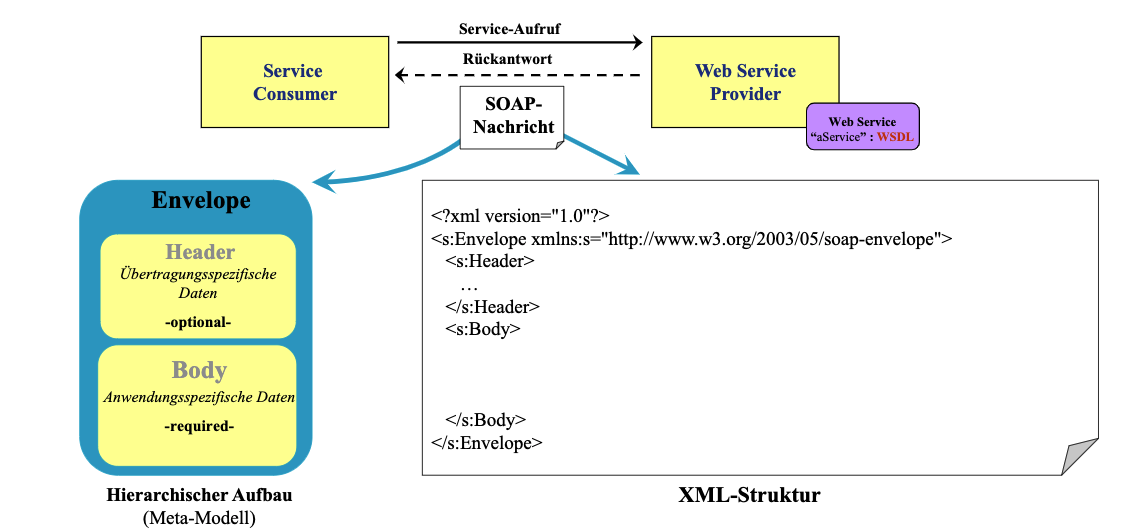
\includegraphics[scale=.4]{images/Struktur_ein_SOAP}
\captionof{figure}{Struktur ein SOAP}
\end{center}

\subsubsection{REST API}
Damit wir die RestFull Api verstehen, fangen wir erst wieder mit den Definitionen ein.
Ein REST stellt einen alternativen Ansatz für die Realisierung von Web Services dar.“ Eine Rest API ist eine Schnittstelle, über die Sie die Kommunikation zwischen Ihrem Computer und einem Server herstellen können, damit dieser Ihnen Daten zur Verfügung stellt. Rest-API ist die an der häufigsten verwendeten Art von API im Webbereich. REST steht für Representational State Transfert.\cite{alda}

\textit{\textbf{Historik}}

Vor den 2000er Jahren gab es keine Standards dafür, wie man eine API entwirft oder gar verwendet. Die Integration von APIs erforderte die Verwendung von Protokollen, wie z. B. SOAP, die notorisch komplex in der Erstellung, Verwaltung und Fehlersuche sind. Das alles änderte sich in den 2000er Jahren, als das wahre Potenzial von Web-APIs erkannt wurde. Eine Gruppe von Experten, angeführt von Roy Fielding, erfand REST und veränderte die API-Landschaft für immer.
Das Ziel war es, einen einfachen Standard zu schaffen, der es zwei Servern ermöglicht, miteinander zu kommunizieren und Daten auszutauschen, egal wo auf der Welt sie sich befinden. Sie schufen eine Reihe von Prinzipien, Eigenschaften und Einschränkungen, die REST genannt werden, sowie eine ressourcen-orientierte Architektur: einheitliche Schnittstelle, Client/Server-Architektur, keines Zustands, Implementierung der Ressourcen-darstellung, Verwendung von HTTP und HTTP-Methoden.

\textit{\textbf{Anwendung}}

Eine API wird oft mit dem Server oder der Datenbank verwechselt, aber in Wirklichkeit handelt es sich um den Code, der den Server anweist, bestimmte Aktionen entsprechend der gestellten Anfrage auszuführen. Es handelt sich also einfach um ein Interface (Application Programming Interface).
Der Zugriff auf den Rest der API erfolgt über HTTP-Methoden (GET, POST DELETE, PUT). Dadurch ist es möglich, einen Server mit einer vom Ersteller der API bereitgestellten URL durch eine einfache HTTP-Anfrage zu interagieren. Eine HTTP-Anfrage an einen Server provoziert jedoch eine Antwort, je nach Erfolg (Code: 200) oder Misserfolg der Operation (403, 404, 500, 504 ...). Es ist möglich, die Daten Allgemeinen im JSON-Format zu erhalten.

\begin{center}
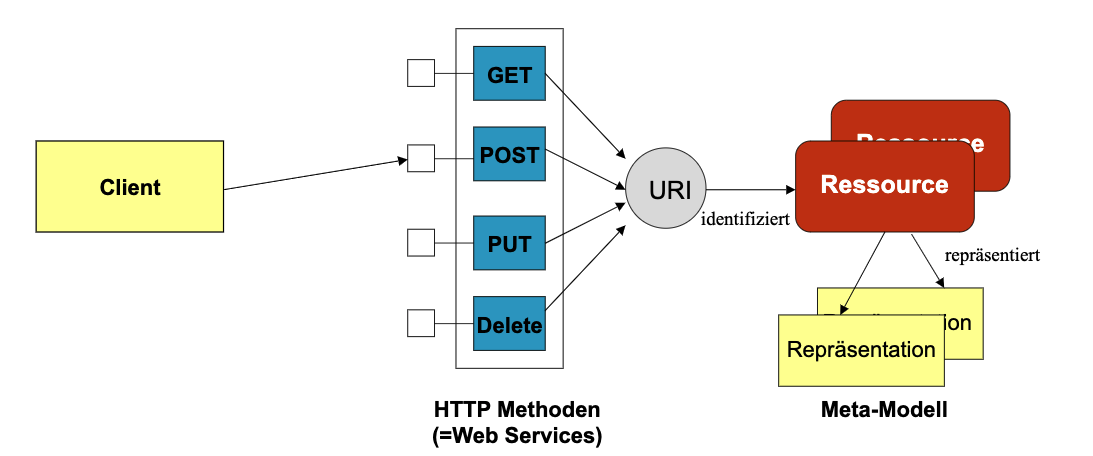
\includegraphics[scale=.3]{images/Aufbau_eine REST-basierten_Web_Services_Architektur}
\captionof{figure}{Aufbau eine REST-basierten Web Services Architektur}
\end{center}

\subsubsection{GraphQL}

GraphQL ist eine Abfragesprache für APIs und eine Laufzeitumgebung zur Erfüllung dieser Abfragen mit Ihren vorhandenen Daten. GraphQL bietet eine vollständige und verständliche Beschreibung der Daten in Ihrer API, gibt Kunden die Möglichkeit, genau das anzufordern, was sie benötigen, und nicht mehr, erleichtert die Weiterentwicklung von APIs im Laufe der Zeit und ermöglicht leistungsstarke Entwicklerwerkzeuge.\cite{graphQL}

\textit{\textbf{Historik}}

Bis 2012 wird die Verbreitung von Mobiltelefonen weltweit monströse Zahlen erreichen. Es ist eine solche Invasion, dass Unternehmen, die ihre Produkte nicht anpassen, gefährdet sind. An diesem Punkt ist Facebook gefährdet. Facebook geht online. Als Ergebnis haben sie ihre IOS-App wie eine Website gemacht, in Web-Ansicht. Sehr schnell merken sie, dass es (zu diesem Zeitpunkt) ein bisschen scheiße ist. Also entschied man sich, es komplett in nativer Sprache neu zu erstellen, um ein besseres Kundenerlebnis zu schaffen. Sofort wurde ihnen eine weitere Wand vor die Nase gesetzt. Die bestehende Architektur funktioniert nicht. Hauptsächlich, weil die Endpunkte ihrer bestehenden REST-API keine Flexibilität bei den Daten zulassen. Für verschachtelte Daten sind mehrere Roundtrips zu verschiedenen Endpunkten erforderlich, was zu Langsamkeit und Inkonsistenzen führt. Ein Teil der Nutzdaten wird für die meisten Abfragen nicht benötigt, was zu unnötigen Datenübertragungen führt. Und vor allem ist es für Facebook mühsam, so viele HTTP-Aufrufe zu verarbeiten.
In diesem infernalischen Kontext reservieren Lee Byron, Dan Schafer und Nick Schrock im Februar 2012 Büros in einer Ecke von Facebook. Sehr schnell wird ein erster Prototyp von GraphQL, damals SuperGraph genannt, von unseren drei Entwicklern erstellt. Im August 2012 wird GraphQL in der Produktion mit der neuen nativen Facebook-App ausgeliefert. Im Jahr 2015 erscheint die erste öffentliche Version im Internet. GraphQL ist auch heute noch präsent, wenn Sie auf Ihrer Facebook-Pinnwand scrollen.\cite{graphQL2}

\textit{\textbf{Anwendung}}

Mit GraphQL kann man Daten auf einfache, flexible und sehr präzise Weise manipulieren. GraphQL ist keine Programmiersprache und kein Framework, sondern eine Spezifikation zur Implementierung einer API.
GrapQL macht das Leben einfacher, denn damit müssen Sie nur eine Post request Anfrage stellen, die nach genau dem fragt, was man genau braucht, als Antwort gibt es die Ressourcen zurück, die nach dem Aufbau Ihres GraphQL Anfrage. Der kleine Unterschied zu REST ist, dass man bei REST von den Endpunkten definierte Objekte bekommt, bei GraphQL hingegen passt man sich nicht an ein vom Backend bereits vordefiniertes Objekt an, sondern man definiert dynamisch, was man auf der Frontend Seite erhalten möchte. 
Das folgende Bild von der Startseite der offiziellen GrapQL-Website stellt die Funktion von GraphQL übersichtlich und einfach dar.

\begin{center}
\includegraphics[scale=.4]{images/Globaler_ueberblick über_GraphQL}
\captionof{figure}{Globaler Überblick über GraphQL}
\end{center}

